\documentclass[10pt, letterpaper]{article}
\usepackage{graphicx}
\usepackage[bottom=1.0in]{geometry}
\topmargin=-0.9in
\oddsidemargin -.3in
\evensidemargin -0.3in
\textwidth=7.0in
%\itemsep= -0.5in
%\parsep= -0.04in

\usepackage[cmex10]{amsmath}
\usepackage{multirow}



\author{Madhusudan Govindraju 39267182 }
\date{}
\begin{document}
\title{EEL5840  Elements of Machine Intelligence - HW 6}
\maketitle

The document explains all the assumptions and the steps undertaken to complete the assignment and the results  are attached. The code implemented to run this assignment is available towards the end of the document.

\textbf{ Steps to decide the Network Configuration}
\begin{enumerate}
\item Every Neural Network has atleast 3 layers. Exactly 1 Input layer, 1 hidden layer, exactly 1 output layer. 
\item The number of processing elements in the hidden layer should not be greater than twice the number of input elements. Generally to start-off we start with a n number of processing elements in the hidden layer, where n is the average of the number of elements of the input layer and output layer(in our case 2 elements)
\item The Input layer has 2 nodes because we have two inputs x1 and x2. In our implementation we will include the bias also as an input. 
\item The Output layer is going to have 1 node because we are implementing a regressor or classifier and It is going to give out just one predicted class.
\item We will consider 3 cases. They are 2 hidden layer nodes, three hidden layer nodes and 4 hidden layer nodes. This is because we first start with one hidden layer and the number of processing elements in the hidden layer equal to the number of neurons in the input layer. If the error is too large then we can try to use a different number of Processing Element in the hidden layer. In addition to this we will use one more bias input in the hidden layer.
\item We start the network with random values in the $W_{ji}$, and $W_{kj}$ matrices and we go on to update these weights after every epoch.
\end{enumerate}

\begin{figure}[h!]
\centering
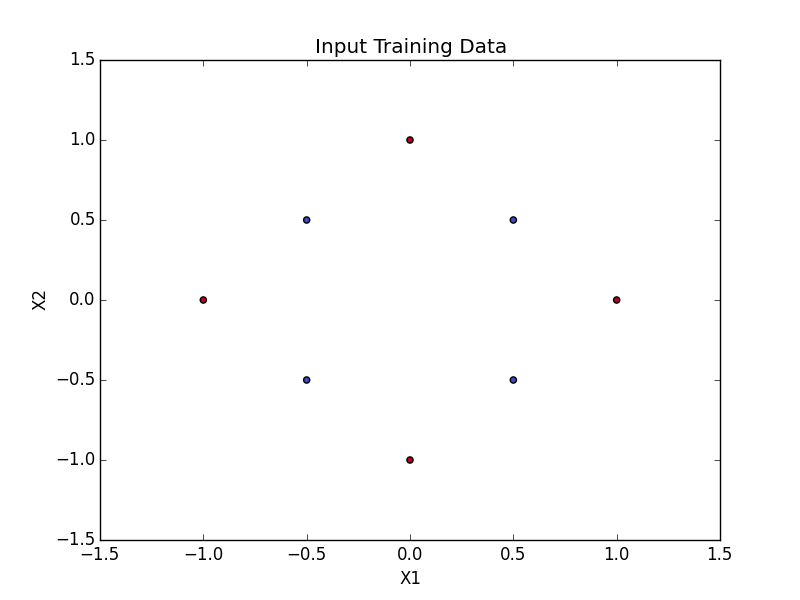
\includegraphics[scale=0.75]{InputData.png}
\caption{Input Training Data}
\label{fig:Input}
\end{figure}



\textbf{Explaining the Implementation}
\begin{enumerate} 
\item First we randomly initialize the weights $W_{ji}$, and $W_{kj}$.
\item Feed forward
\begin{verbatim}
l0 = X
l1 = sigma(np.dot(l0, Wji))
l2 = sigma(np.dot(l1, Wkj))
\end{verbatim}
Here the the l0, l1, l2 are the outputs of the activation functions from the input,  hidden and output layers respectively.
\item Next is the back propogation
\begin{verbatim}
# this is the Error of the system (Final output error)
l2_error = y - l2 
#this corresponds to delK
l2_delta = l2_error * sigma_deriv(l2)
#this corresponds to the value that should be added to the Wkj
del_Wkj = l1.T.dot(l2_delta)
# this is the error of the hidden layer
l1_error = l2_delta.dot(Wkj.T)
#this corresponds to delJ
l1_delta = l1_error * sigma_deriv(l1)
#this corresponds to the value that should be added to the Wji
del_Wji = l0.T.dot(l1_delta)
\end{verbatim}
\item Next is to update the weights
\begin{verbatim}
#updating the weights with respect to the learning rate
Wkj += del_Wkj *epsilon
Wji += del_Wji *epsilon
\end{verbatim}

\item After training we give a few points in the same sample space defined by -1 to +1 and check the outputs of the neural network
\begin{verbatim}
#generate data to check the decision boundary
h = .1 #the step size in the mesh plot
x_min, x_max = X[:, 0].min() - 1, X[:, 0].max() + 1
y_min, y_max = X[:, 1].min() - 1, X[:, 1].max() + 1
xx, yy = np.meshgrid(np.arange(x_min, x_max, h),
                     np.arange(y_min, y_max, h))
inp = np.c_[xx.ravel(), yy.ravel(),np.ones(len(xx.ravel()))]
Z = predict_self(inp,Wji,Wkj)
Z = Z.reshape(xx.shape)
plt.contourf(xx, yy, Z, cmap=plt.cm.coolwarm, alpha=0.8)
plt.scatter(X[:, 0], X[:, 1], c=y, cmap=plt.cm.coolwarm)
plt.xlabel('X1')
plt.ylabel('X2')
plt.xlim(xx.min(), xx.max())
plt.ylim(yy.min(), yy.max())
plt.show()
\end{verbatim}

\end{enumerate}

\textbf{Observations}
\begin{enumerate}
\item \textbf{Case1} In this we implement the Neural Network with 2 hidden layer nodes. So the structure is going to be as shown in the figure \ref{fig:Case1}
\begin{figure}[h!]
\centering
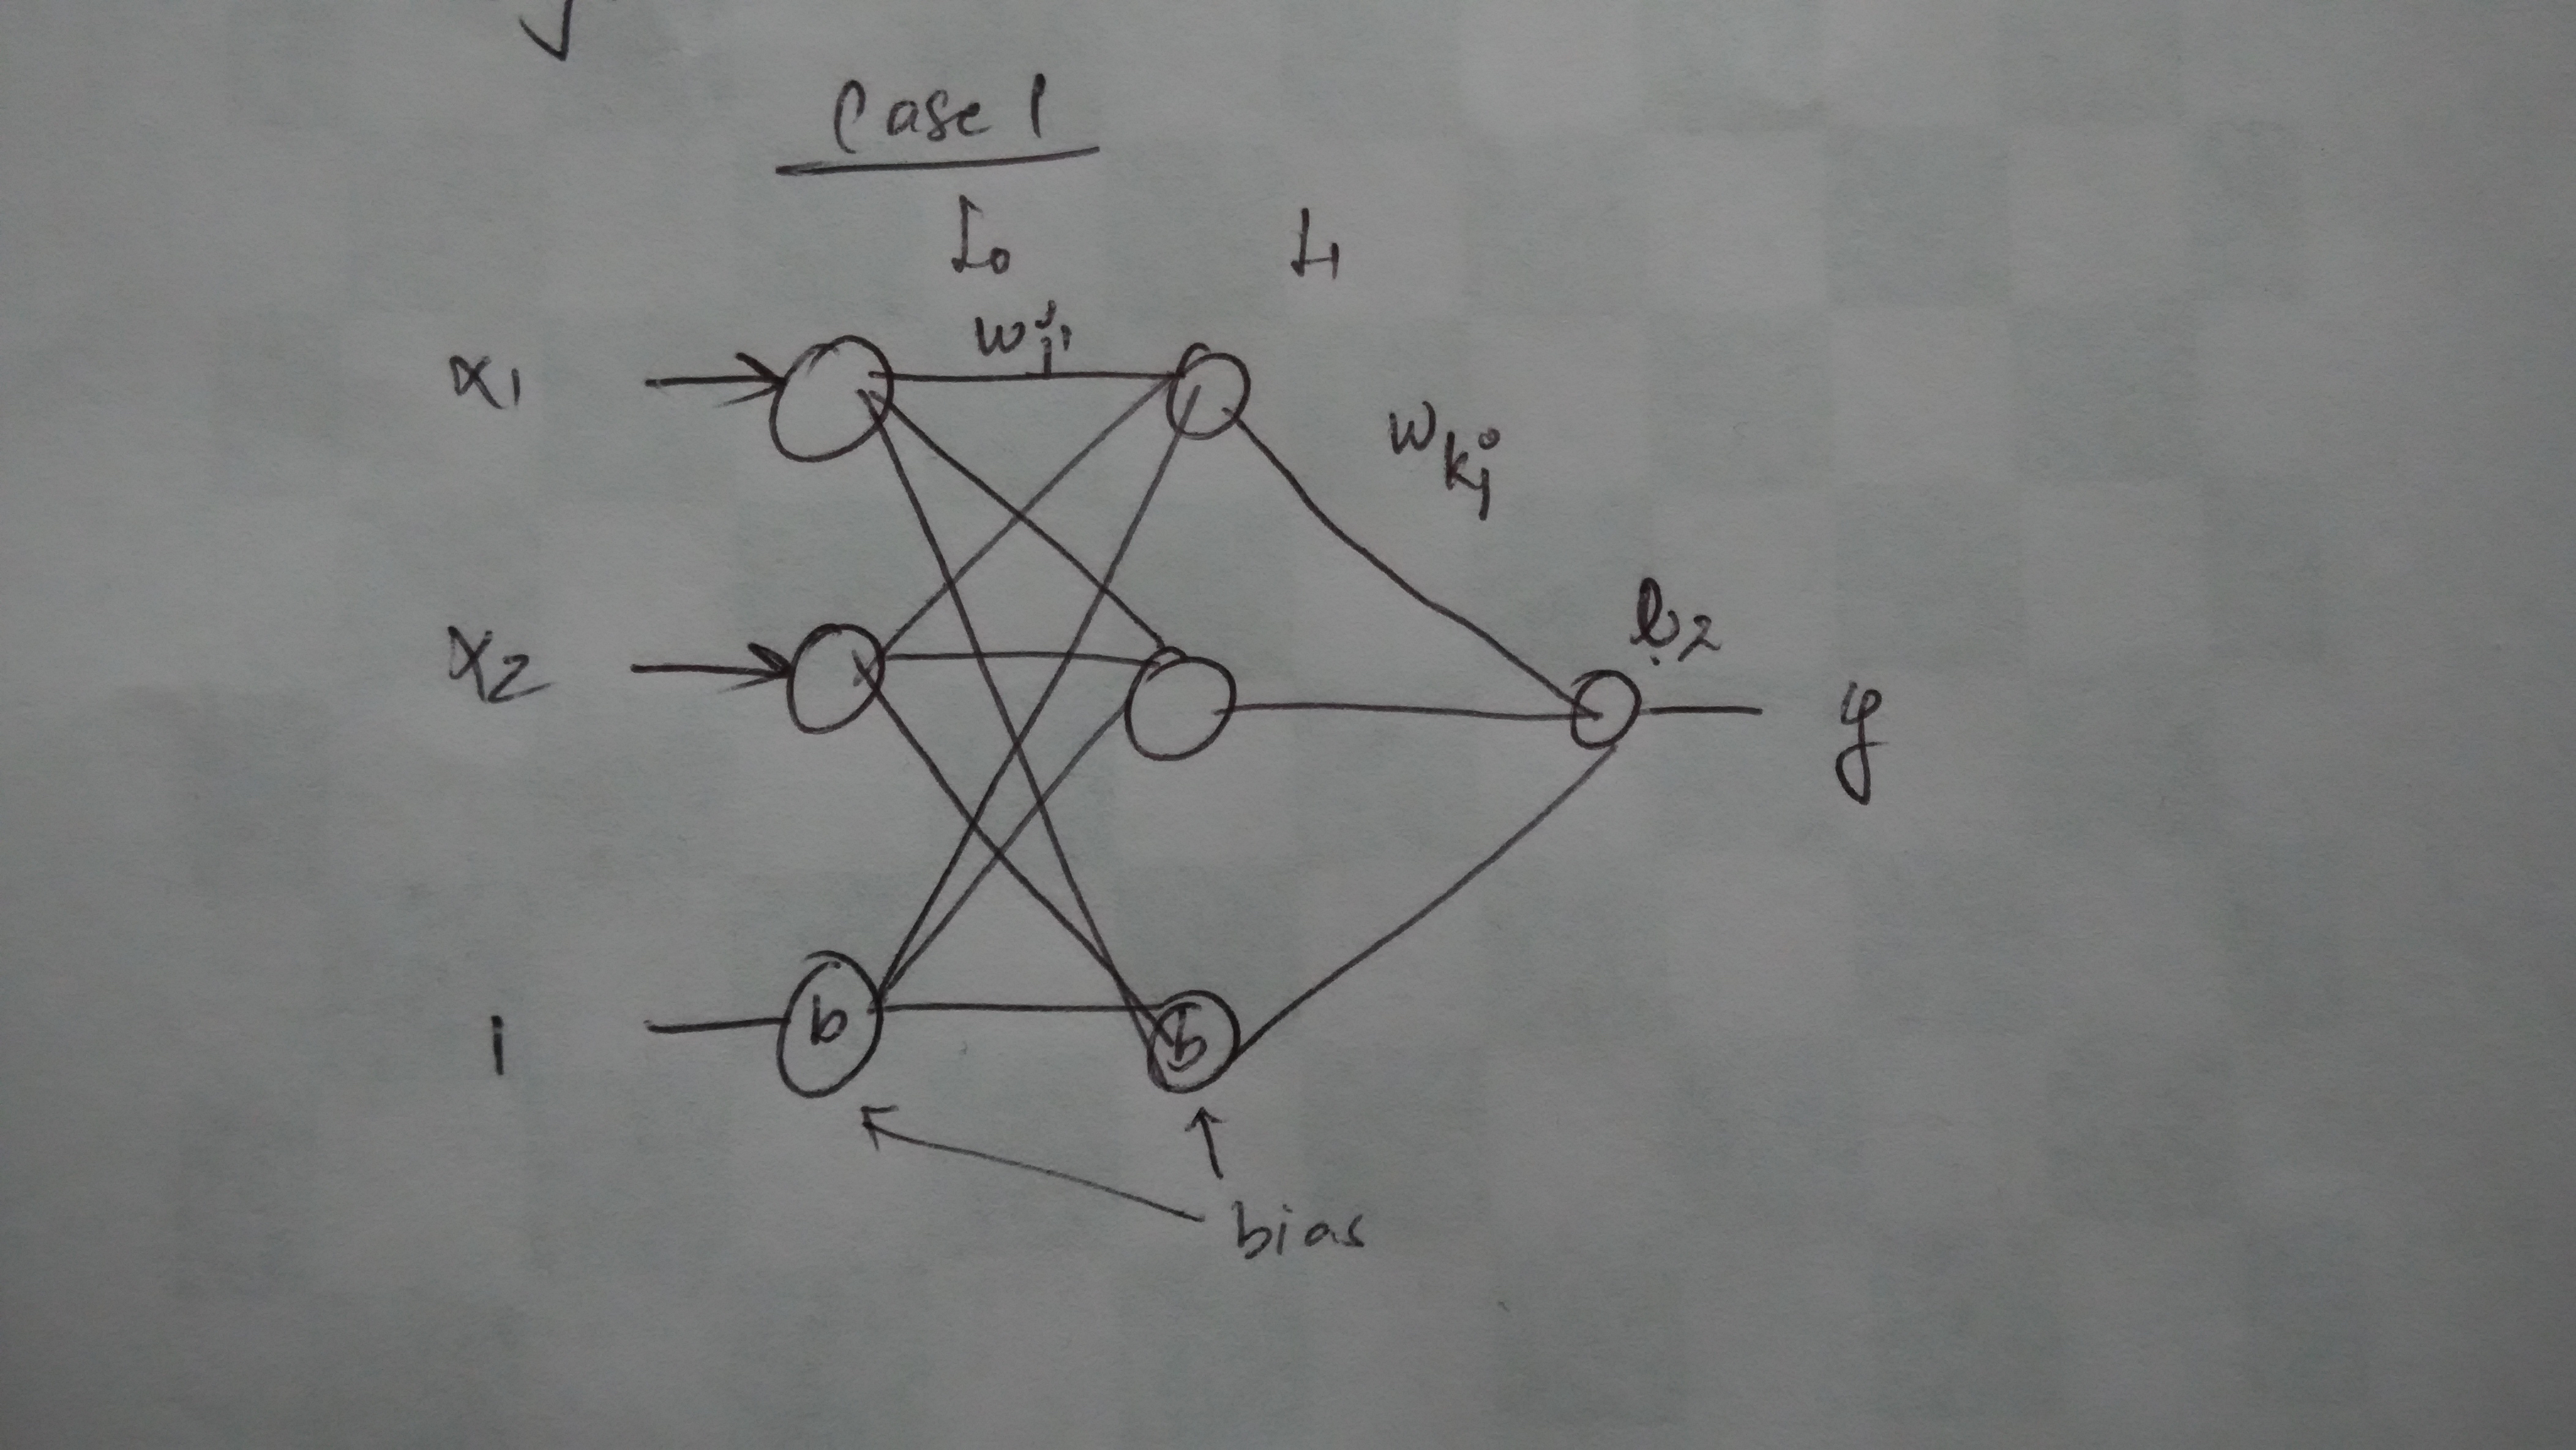
\includegraphics[scale=0.1]{case1.jpg}
\caption{Case1}
\label{fig:Case1}

\centering
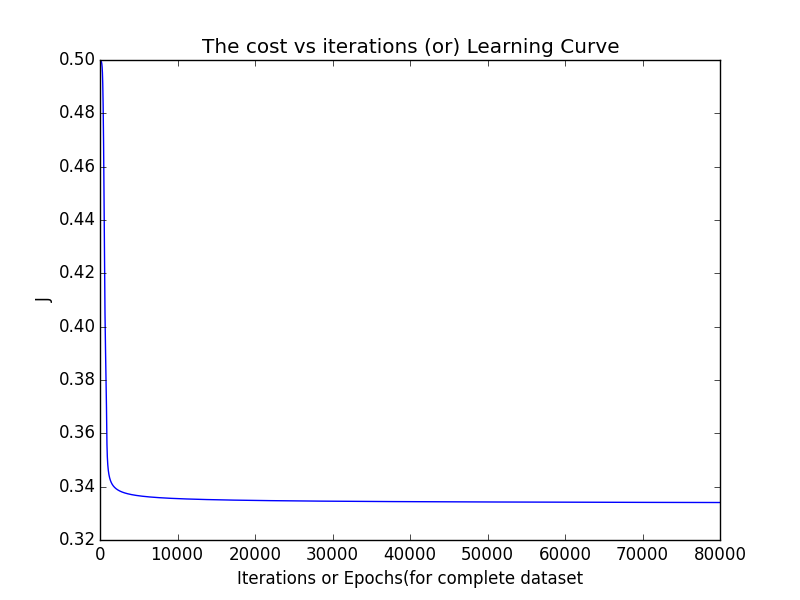
\includegraphics[scale=0.5]{3_3_1_learning.png}
\caption{Case1 - Learning Rate}
\label{fig:LR1}

\centering
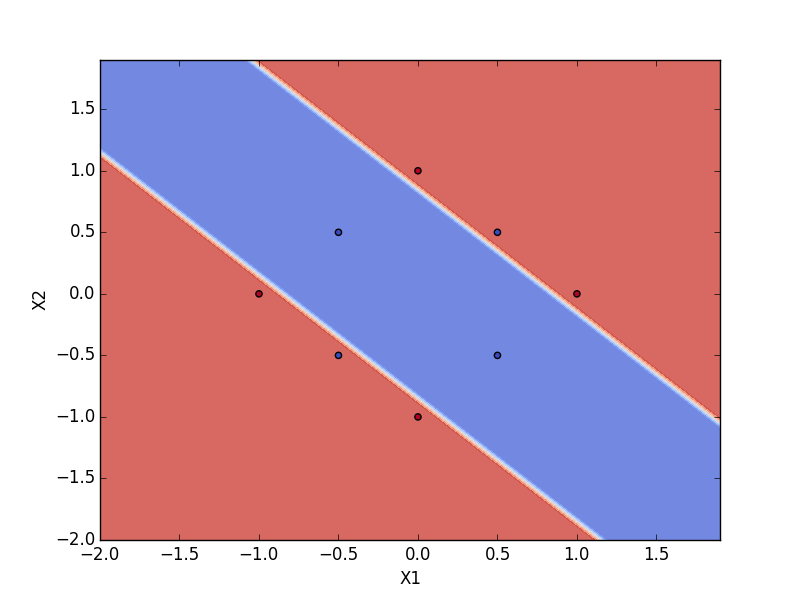
\includegraphics[scale=0.5]{3_3_1.png}
\caption{Case1 - Decision Boundary}
\label{fig:d1}
\end{figure}
The error is very high in this case, This can be seen clearly in the learning curve. Shown in the figure \ref{fig:LR1} .The decision boundary for the input space can be viewed in the fig \ref{fig:d1}. The Error does not go below than 0.34 which is quite high. as we can see in the decision boundary that constantly 2 point will be mis-classified. So we go to the next step to increase the number of processing elements in the hidden layer as we can clearly see 2 elements are not enough.








\item \textbf{Case2}: This case has 3 hidden elements. The diagram of the netework can be checked in the figure \ref{fig:Case2}. The error seems to have reached the lowest possible (Error = 0.00468195642503). This can be seen in the learning rate fig \ref{fig:LR2}. And the decision boundary can be checked in the fig \ref{fig:d2}. We can see that all the points have been classified properly. There seems to be no problem. But we can see that one arm of the decision boundary seems to have been cut off. So we proceed to the next case by adding one more hidden layer processing element.

\begin{figure}[h!]
\centering
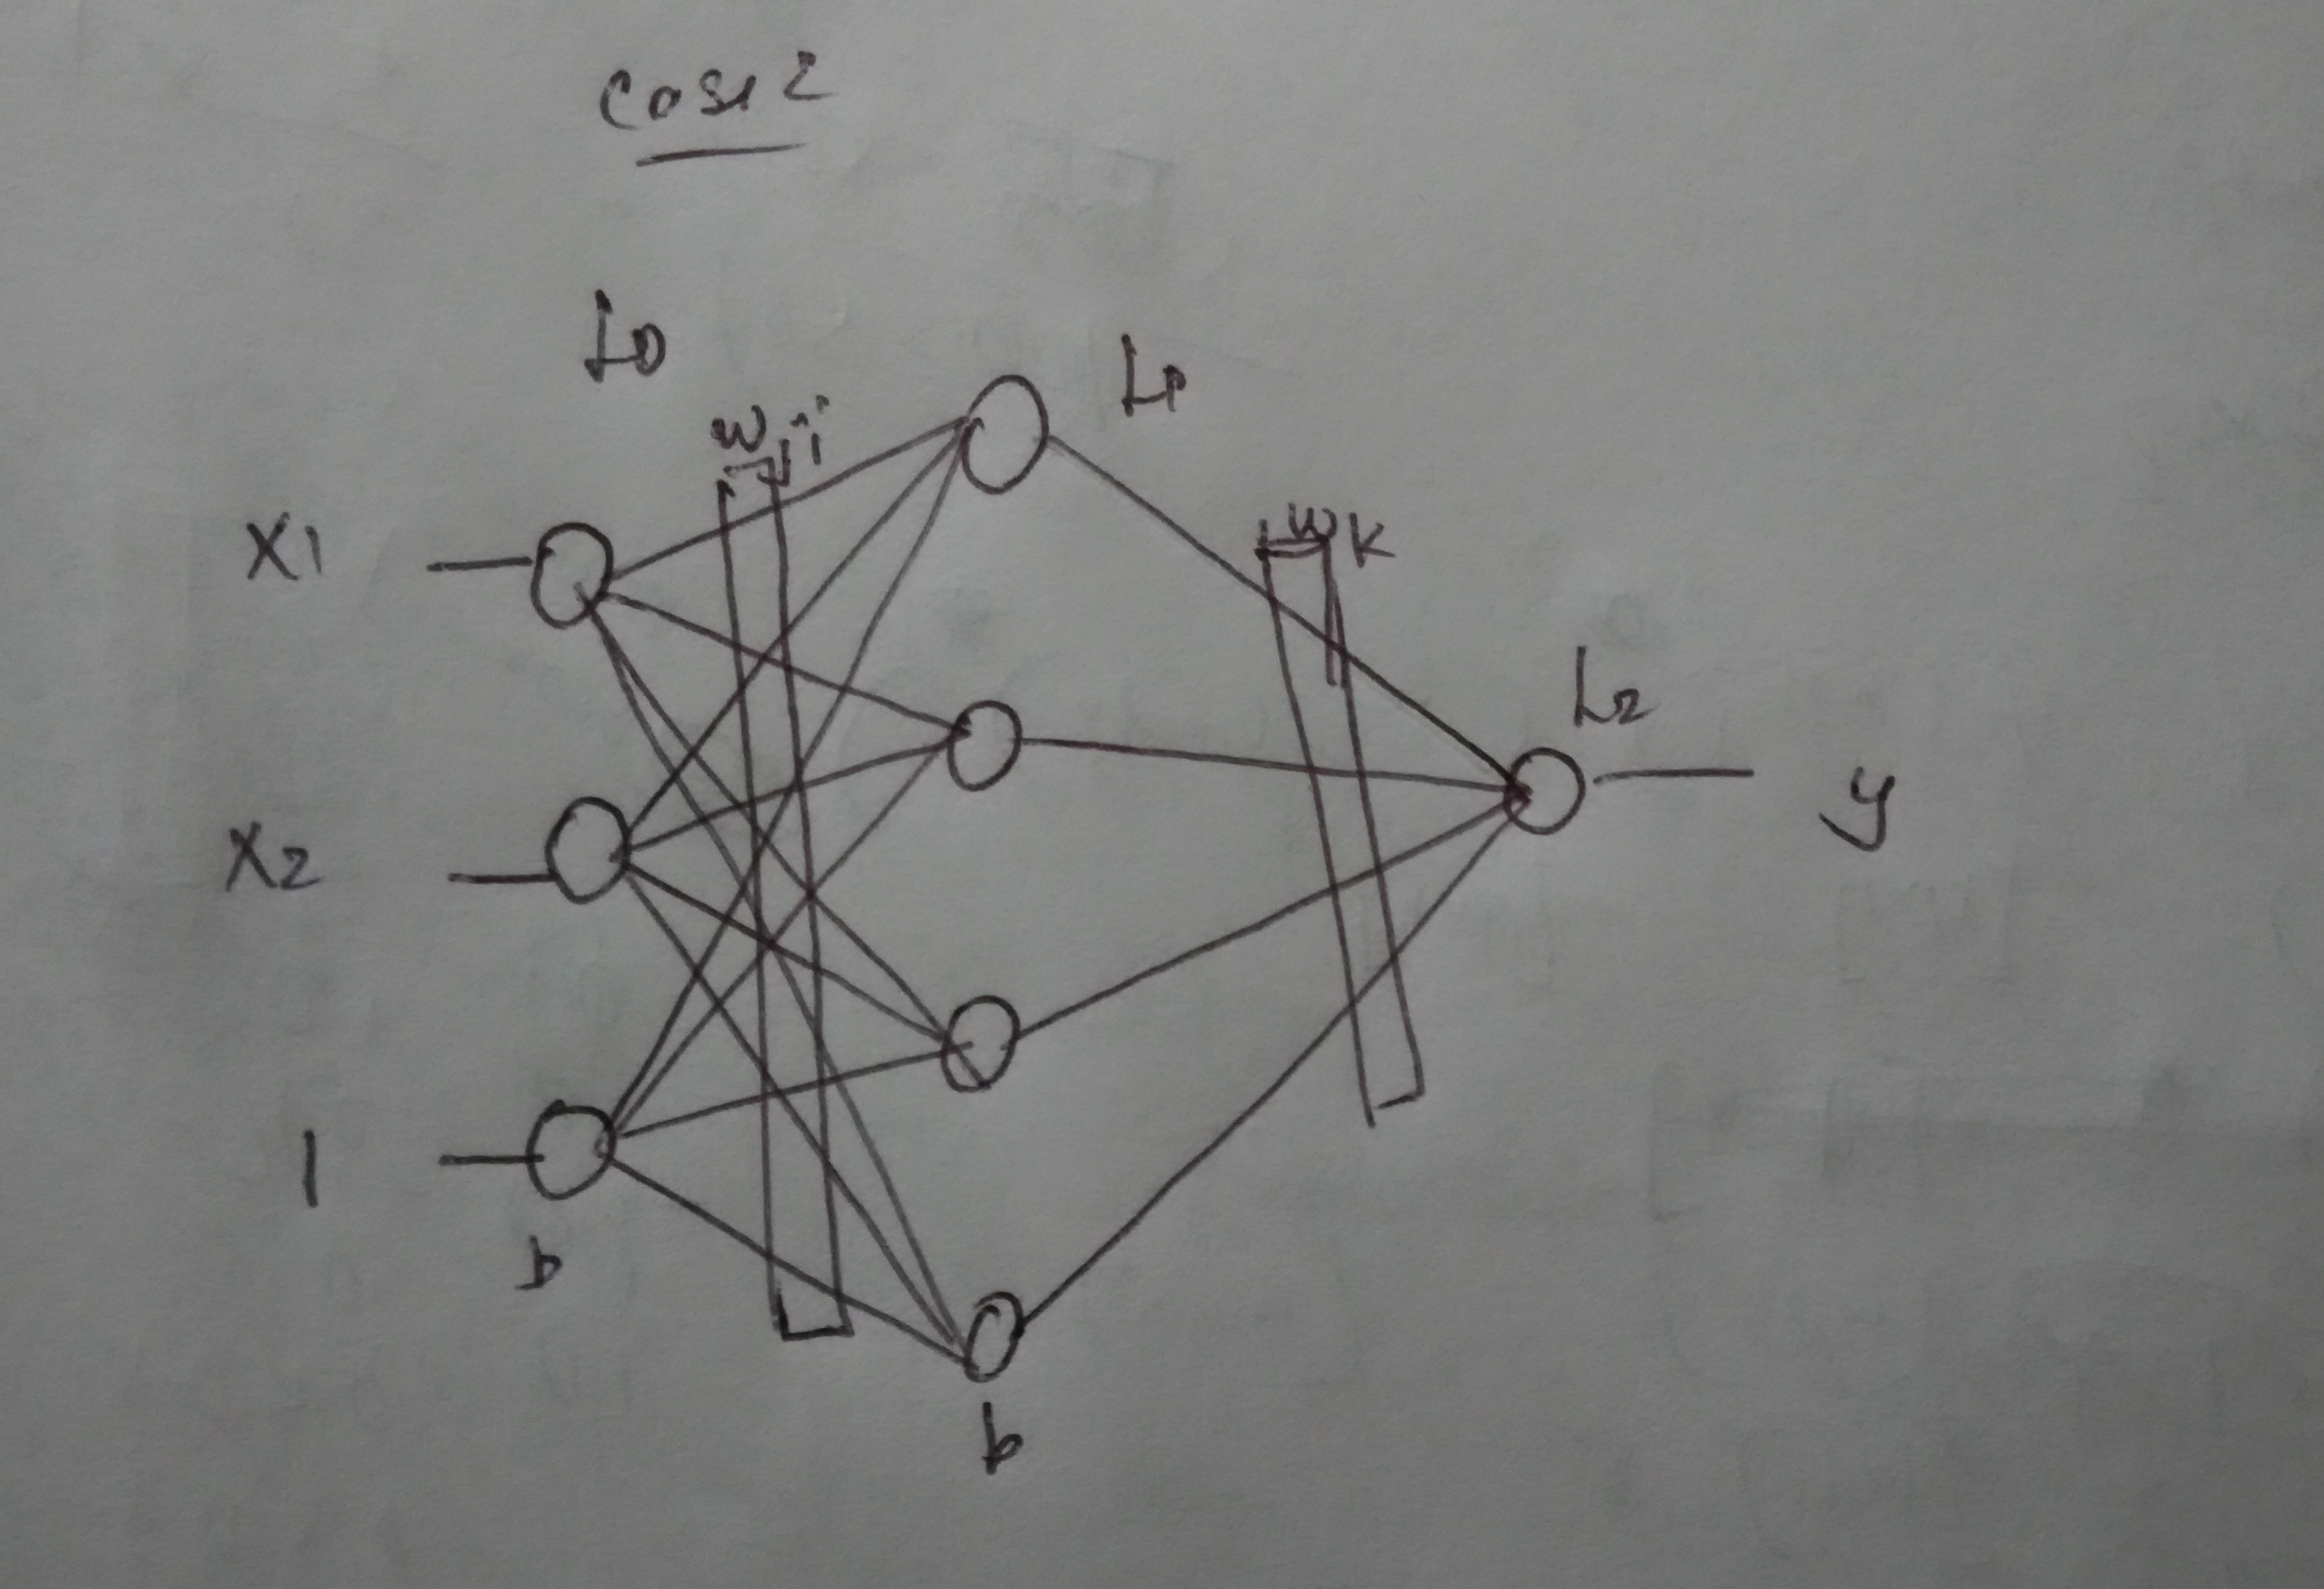
\includegraphics[scale=0.1]{case2.jpg}
\caption{Case2}
\label{fig:Case2}

\centering
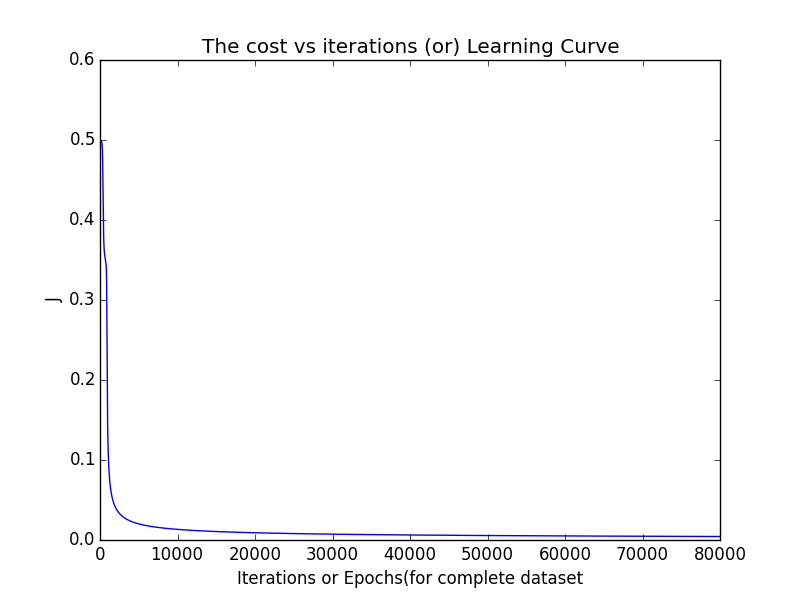
\includegraphics[scale=0.5]{3_4_1_learning.png}
\caption{Case2 - Learning Rate}
\label{fig:LR2}

\centering
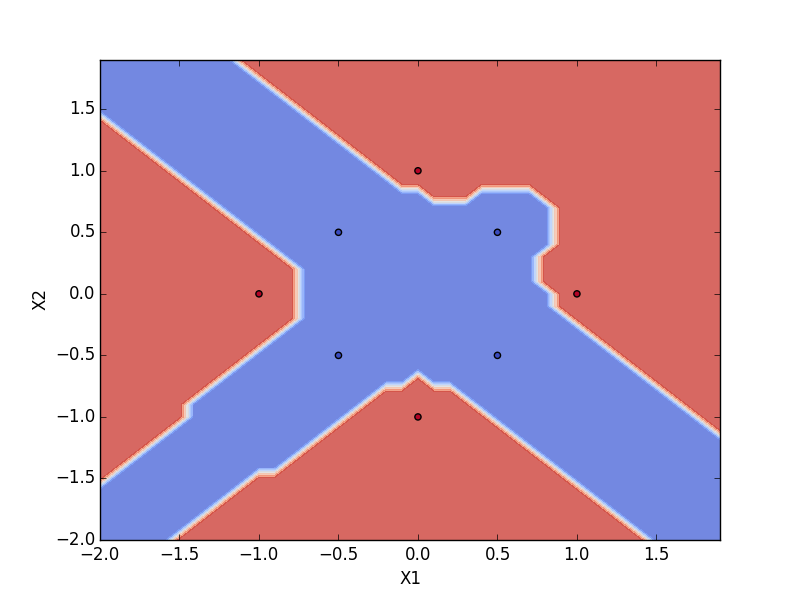
\includegraphics[scale=0.5]{3_4_1.png}
\caption{Case2 - Decision Boundary}
\label{fig:d2}
\end{figure}

\item \textbf{Case 3}: This seems to be the best case with the least error rate at Error:0.00404925847779. We can see that there is not much change considering the case 2. But when we check the decision boundary we can identify there is another decision boundary for the point along the positive x-axis. This confirms our decision boundary. All the points near the major axis should be classified as 1 and all the other points away from the 4 major axis should be classified as 0. We can see than the decision boundary will join wth each other at infinity and group all the points near the 4 major axis as class 1.

\begin{figure}[h!]
\centering
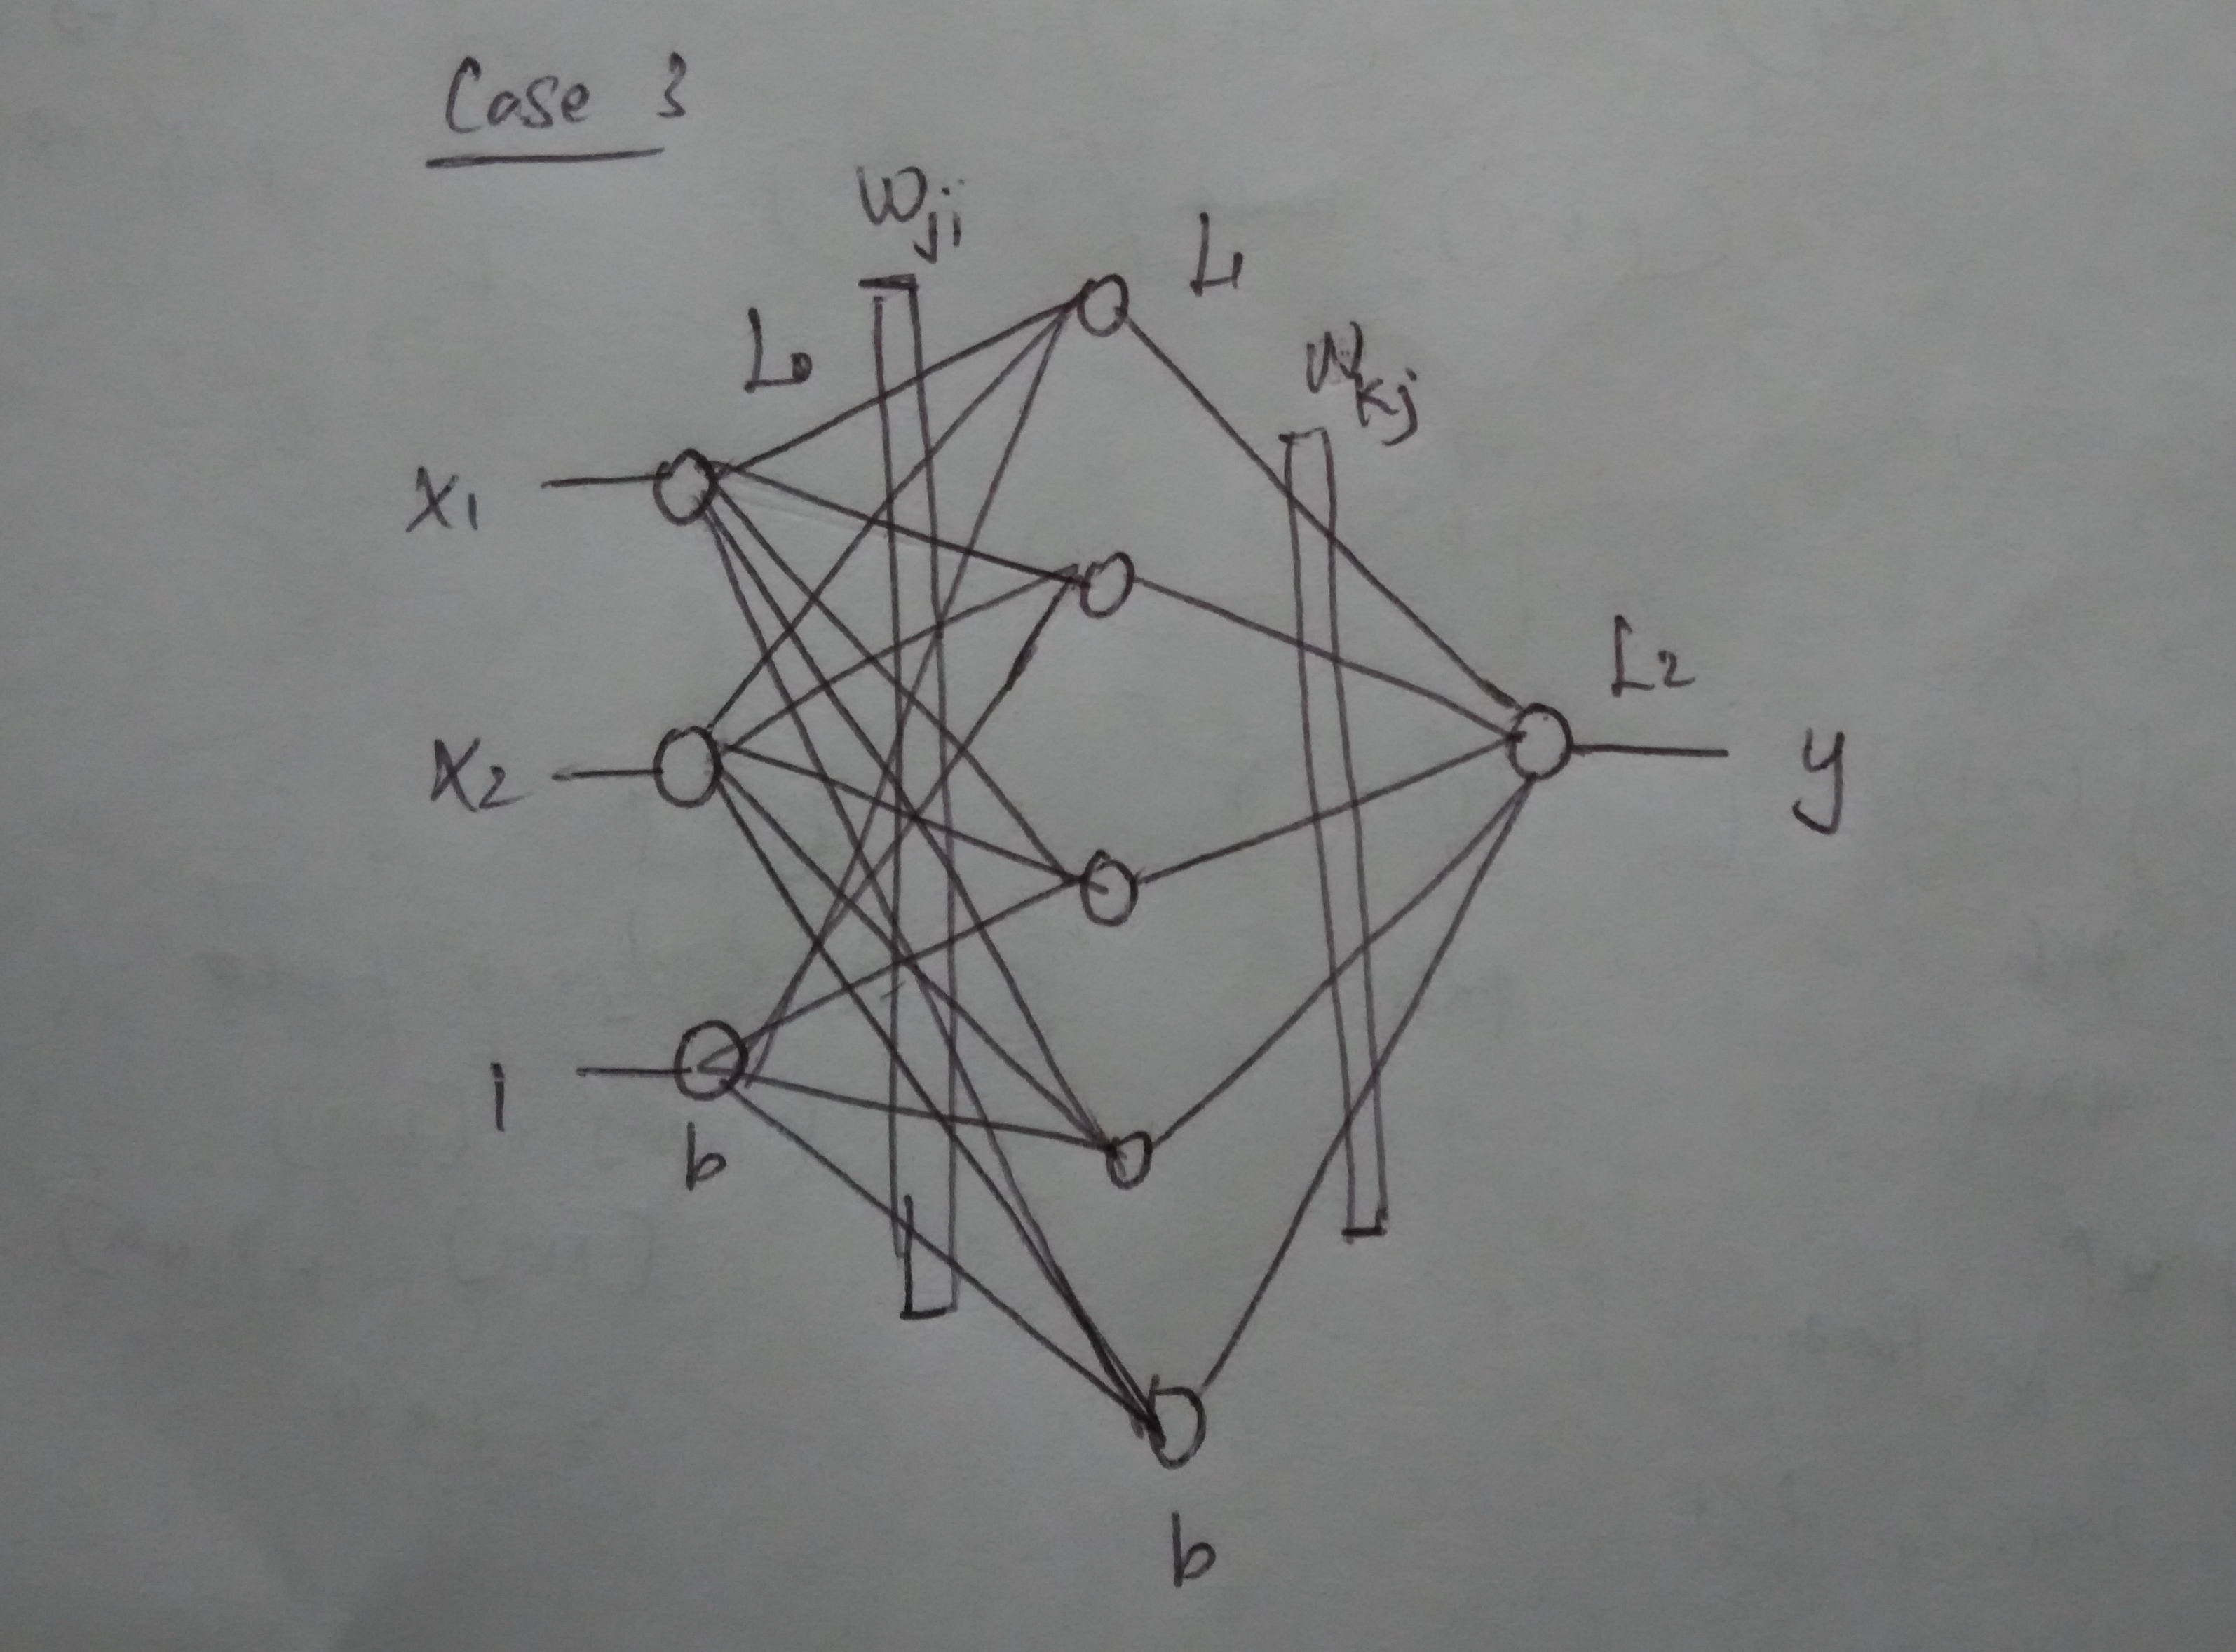
\includegraphics[scale=0.1]{case3.jpg}
\caption{Case3}
\label{fig:Case3}

\centering
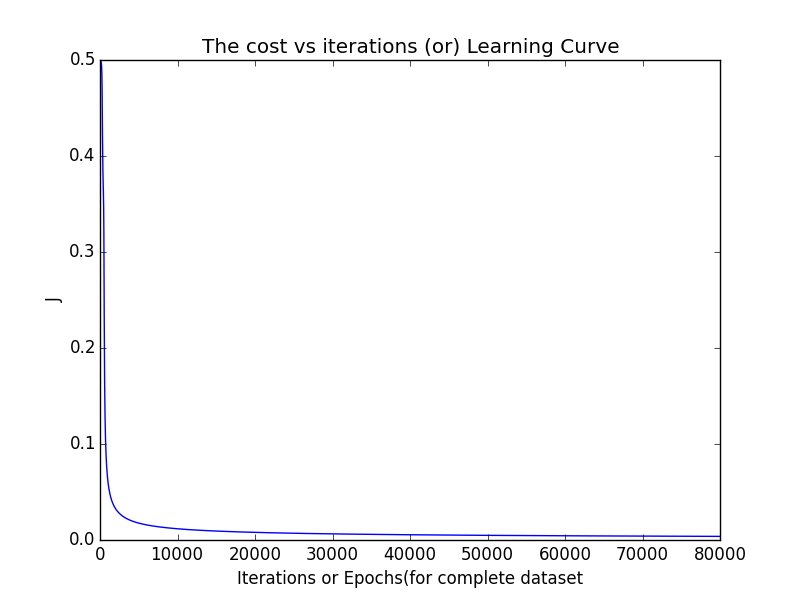
\includegraphics[scale=0.5]{3_5_1_learning.png}
\caption{Case3 - Learning Rate}
\label{fig:LR3}

\centering
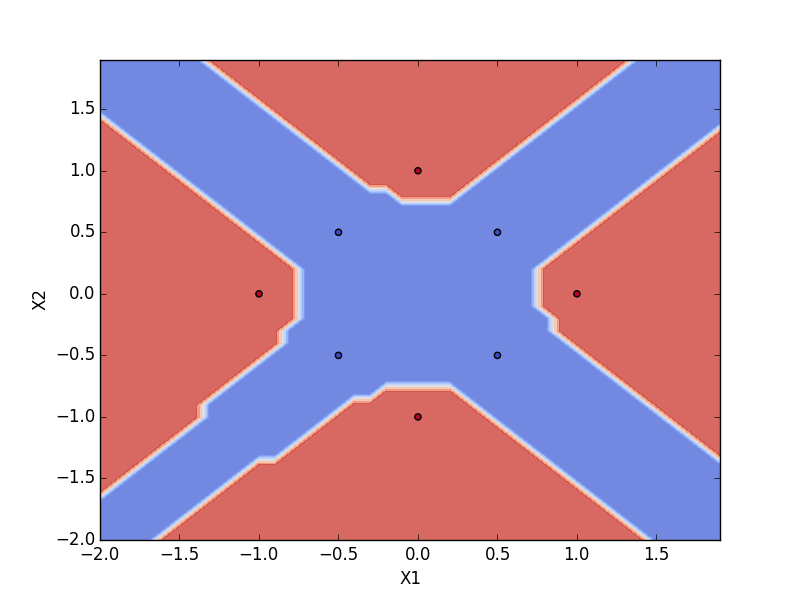
\includegraphics[scale=0.5]{3_5_1.png}
\caption{Case3 - Decision Boundary}
\label{fig:d3}
\end{figure}

\item For more number of hidden layer processing elements we check the error reduces ,ie., for 7 hidden layer elements, the error = 0.0038650526305 but, the decision boundary does not change any more. Only the points very close to the decision boundary may be classified into the wrong class, But our training samples can be classified 100\% so adding more training samples might help in forming a more complex decision boundary, but the number of the 

\item For more number of hidden layer processing elements the error reduces ( for 7 PE error=0.0038650526305), but there is no change in decision boundary , even for 20 processing elements in hidden layer. From this we can conclude that 5 is the ideal number of processing elements required in the hidden layer for obtaining the required decision boundary. With more training samples we might get a more complex or simpler decision boundary(this is based on the input training samples). 
\begin{figure}[h!]
\centering
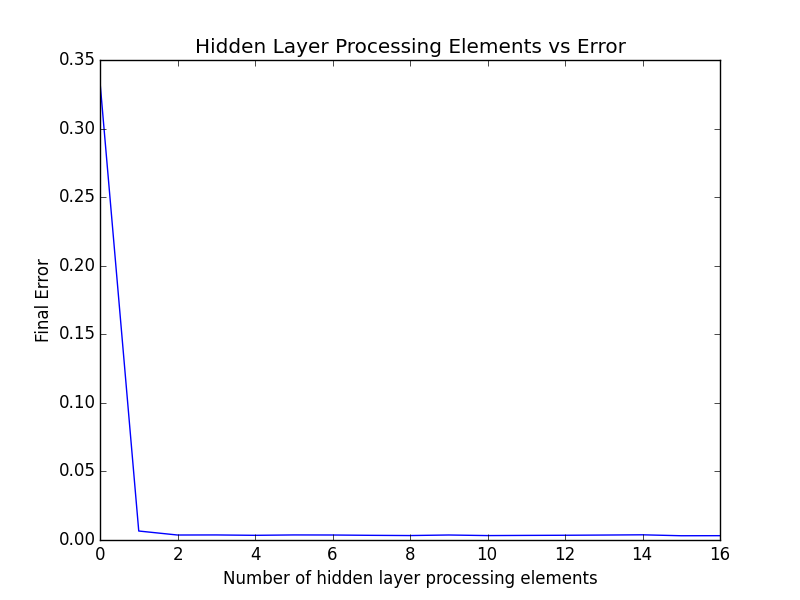
\includegraphics[scale=0.75]{ErrorvsPE.png}
\caption{Error VS Processing Elements, the X axis should be added with a scale of $+3$}
\label{fig:Error}
\end{figure}

\item From the figure \ref{fig:Error} we can see that the error does not change a lot after 5 processing elements. so adding more elements to the hidden layer is not going to increase the efficiency of the system. So the idle point should be 5 processing elements in the hidden layer.

\item We have to chose a 
\begin{figure}[h!]
\centering
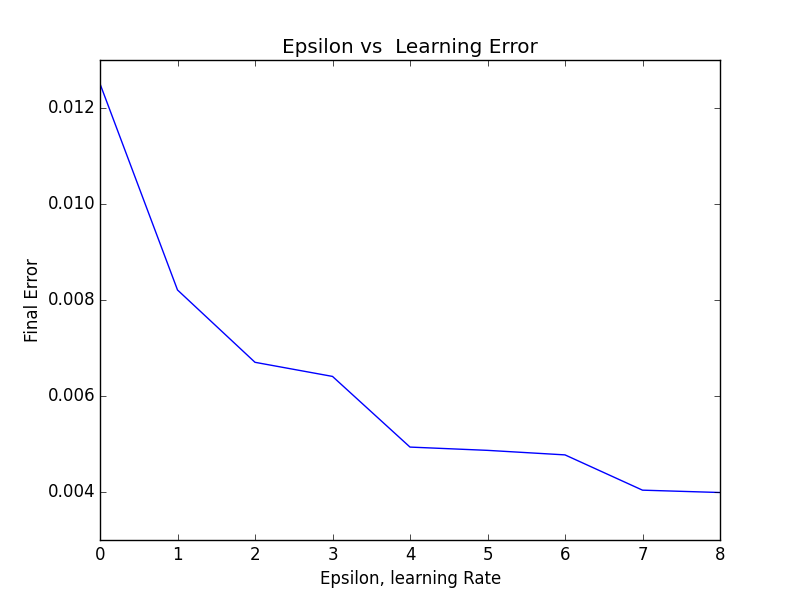
\includegraphics[scale=0.75]{EpsilonvsError.png}
\caption{Epsilon vs Error, here scale the X axis as follows  epsilon/10 + 1}
\label{fig:Epsilon}
\end{figure}

\item From the figure \ref{fig:LearningRate} we can check that as we increase the rate from 0.3 to 0.9 the learning converges faster. Thus choosing the epsilon which gives the best learning convergence is better.
\begin{figure}[h!]
\centering
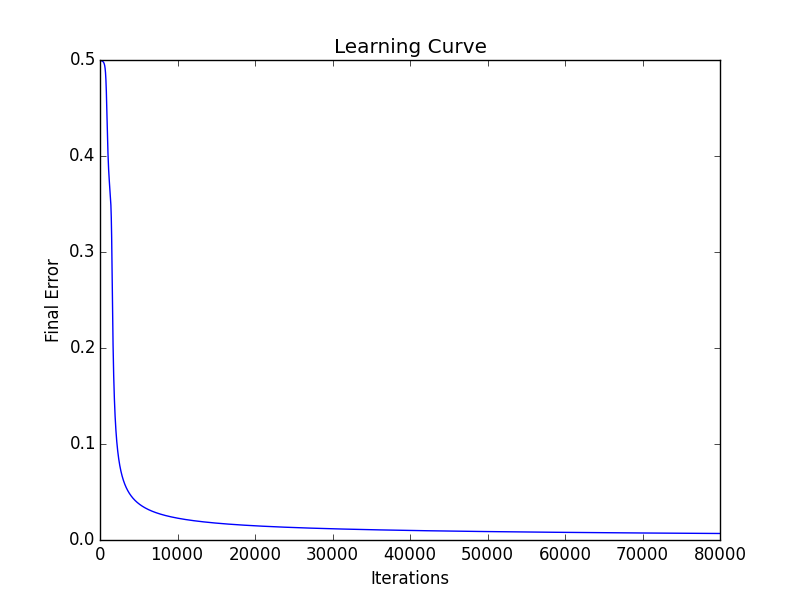
\includegraphics[scale=0.5]{epsilonpt3}
\caption{For epsilon = 0.3}
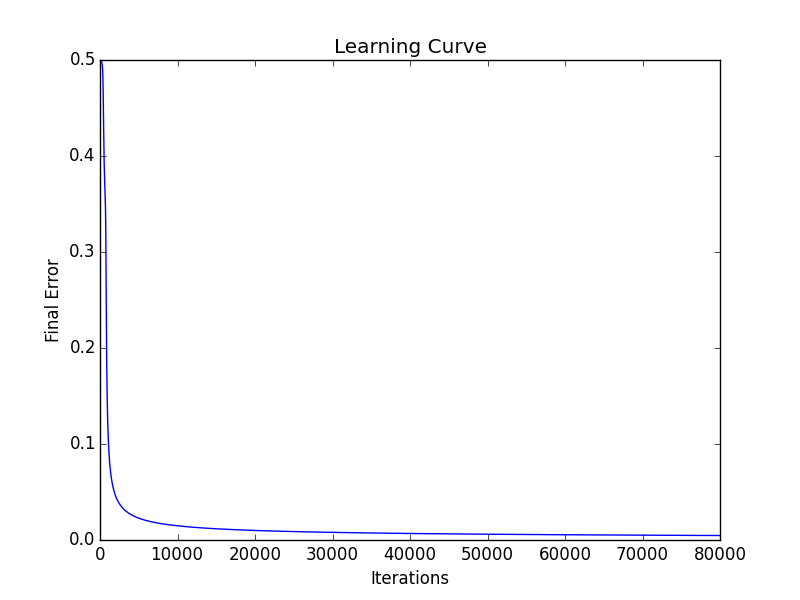
\includegraphics[scale=0.5]{epsilonpt6}
\caption{For epsilon = 0.6}
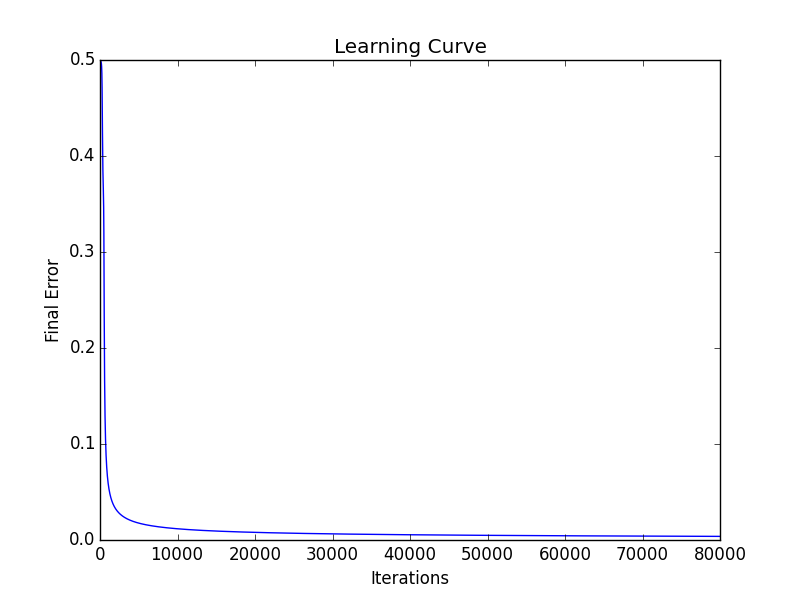
\includegraphics[scale=0.5]{epsilonpt9}
\caption{For epsilon = 0.9}
\caption{Learning Curve}
\label{fig:LearningRate}
\end{figure}


\end{enumerate}

\textbf{Conclusion}
\begin{enumerate}
\item We choose 4 nodes in the hidden layer because each node corresponds to one of the lines bounding the non- convex region.
\item \textbf{To select the parameters of the network}
From the different cases we can also see that the number of processing elements in the hidden layer is equal to the number of decision boundaries. So From the input data as shown in the fig \ref{fig:Input}  we can see that the number of decision boundaries required to properly classify the input data is 4 . So we need 4 elements in the hidden layer to classify the data. 
\item Deducting from the fig \ref{fig:LearningRate} we can assume that increasing the epsilon value reduces the converging time. Hence choosing 0.9 for epsilon is best is best.
\item The multilayered Neural Network learns the solutions properly.
\item The accuracy can be increased by increasing the number of hidden layer elements, but that is going to increase the accuracy only by a small factor for the given set of inputs. The accuracy can be increased by giving more training data to the network during the training phase.  A training data encompasses the extreme points and which defines the decision boundary very accurately is required to get higher accuracy, since the boundaries are completely defined by the training data. 
\end{enumerate}
\newpage
\textbf{The implementation Code}
\begin{verbatim}
import numpy as np
import cv2
import matplotlib.pyplot as plt


def predict_self(inp,wji,wkj):

    l0 = inp
    l1 = sigma(np.dot(l0, wji))
    l2 = sigma(np.dot(l1, wkj))
    l2 = abs(l2)
    out = l2;
    for i in range(len(inp)):
        if l2[i]>0.5:
            out[i]=1
        elif l2[i]<0.5:
            out[i]=0
    return out



def sigma(x, deriv=False):
    return 1 / (1 + np.exp(-x))

def sigma_deriv(x):
    return x * (1 - x)

X = np.array([[1,0,1],
             [0,1,1],
             [-1,0,1],
             [0,-1,1],
             [0.5,0.5,1],
             [-0.5,0.5,1],
             [0.5,-0.5,1],
             [-0.5,-0.5,1]
])

y = np.array([
    [1],
    [1],
    [1],
    [1],
    [0],
    [0],
    [0],
    [0],
])

num_inputs = 3 #2 inps includgin the bias
num_HLNodes = 5 #number of nodes in the hidden layer3
num_out = 1 #number of output nodes
eta = 0.9 #learning rate
Error = [] #a list to store the errors so that we can plot it
np.random.seed(1)

# for z in range(1,10,1):
z = 0.9
# randomly initialize our weights with mean 0
Wji = 2 * np.random.random((num_inputs, num_HLNodes)) - 1
Wkj = 2 * np.random.random((num_HLNodes, num_out)) - 1
for j in range(80000):
    # Feed forward through layers 0, 1, and 2
    l0 = X
    l1 = sigma(np.dot(l0, Wji))
    l2 = sigma(np.dot(l1, Wkj))
    # the error of the output
    l2_error = y - l2
    Error.append(np.mean(np.abs(l2_error)))
    # if (j % 10000) == 0:
    #     print ("Error:" + str(np.mean(np.abs(l2_error))))

    # # to print the Error Plot
    # if (j == 79999):
    #     Error.append(np.mean(np.abs(l2_error)))

    # Backpropogation
    l2_delta = l2_error * sigma_deriv(l2)
    del_Wkj = l1.T.dot(l2_delta)
    l1_error = l2_delta.dot(Wkj.T)
    l1_delta = l1_error * sigma_deriv(l1)
    del_Wji = l0.T.dot(l1_delta)

    # updating the weights with respect to the learning rate
    Wkj += del_Wkj * eta
    Wji += del_Wji * eta



print ("After training")



# create a mesh to plot in
h = .1 #the step size in the mesh plot
x_min, x_max = X[:, 0].min() - 1, X[:, 0].max() + 1
y_min, y_max = X[:, 1].min() - 1, X[:, 1].max() + 1
xx, yy = np.meshgrid(np.arange(x_min, x_max, h),
                     np.arange(y_min, y_max, h))
inp = np.c_[xx.ravel(), yy.ravel(),np.ones(len(xx.ravel()))]
Z = predict_self(inp,Wji,Wkj)
Z = Z.reshape(xx.shape)
plt.contourf(xx, yy, Z, cmap=plt.cm.coolwarm, alpha=0.8)
plt.scatter(X[:, 0], X[:, 1], c=y, cmap=plt.cm.coolwarm)
plt.xlabel('X1')
plt.ylabel('X2')
plt.xlim(xx.min(), xx.max())
plt.ylim(yy.min(), yy.max())
plt.show()

# to plot the J vs Epocs
# plt.plot(Error)
# plt.xlabel('Iterations or Epochs(for complete dataset')
# plt.ylabel('J')
# plt.title('The cost vs iterations (or) Learning Curve')
# plt.show()

#Error vs Hidden Layer PE
# yaxis = [i for i in range(3,20,1)]
# plt.plot(Error,yaxis)
# plt.xlabel('Number of hidden layer processing elements')
# plt.ylabel('Final Error')
# plt.title('Hidden Layer Processing Elements vs Error')
# plt.show()

# #Error vs Epsilon plot
# plt.plot(Error)
# plt.xlabel('Epsilon, learning Rate')
# plt.ylabel('Final Error')
# plt.title('Epsilon vs  Learning Error')
# plt.show()

#Input Data plot
# plt.scatter(X[:, 0], X[:, 1], c=y, cmap=plt.cm.coolwarm)
# plt.xlabel('X1')
# plt.ylabel('X2')
# plt.title('Input Training Data')
# plt.show()

# # Error vs Epsilon plot
# plt.plot(Error)
# plt.xlabel('Iterations')
# plt.ylabel('Final Error')
# plt.title('Learning Curve')
# plt.show()
\end{verbatim}



\end{document}